\section{Teammate-order invariance and how to obtain it}
\label{sec:method}

\begin{figure}[t]
\centering
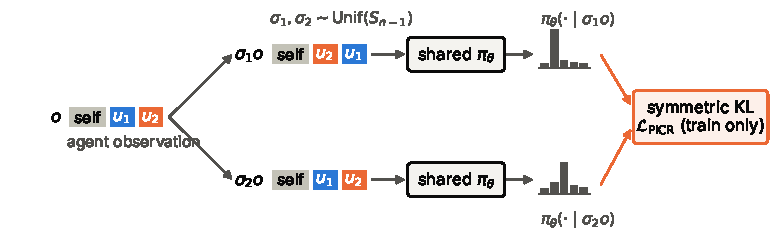
\includegraphics[width=\linewidth]{figures/method_overview.pdf}
\caption{\picr. The teammate blocks of an observation are reordered by two
independent random permutations; the shared policy is applied to both views and
the symmetric KL divergence between the two action distributions is added to the
PPO loss. The penalty is used only during training.}
\label{fig:method}
\end{figure}

\paragraph{Setting.}
We consider $n$ cooperating agents that share one policy $\pi_\theta$
(parameter sharing, \citealp{dewitt2020ippo,yu2022mappo}). Agent $i$'s
observation is $o_i = [s_i, u_{i,1}, \dots, u_{i,n-1}]$, where $s_i$ holds the
agent's own features and the environment, and $u_{i,k}$ is a fixed-width block
of features describing the $k$-th other agent (here, its relative position).
Teammates are exchangeable, so for any permutation $\sigma$ of the $n-1$ blocks
the observation $\sigma o_i = [s_i, u_{i,\sigma(1)}, \dots, u_{i,\sigma(n-1)}]$
describes the same situation. A policy is \emph{teammate-order invariant} if
$\pi_\theta(\cdot \mid \sigma o) = \pi_\theta(\cdot \mid o)$ for all $\sigma$.
An MLP over the concatenated observation has no reason to be invariant: the
slot a teammate occupies is determined by agent indices, so the policy can
learn conventions keyed to ``the first teammate''.

\paragraph{Methods.}
We compare four ways of handling teammate order, all trained with the same PPO
learner and hyperparameters:
\begin{itemize}[leftmargin=1.3em,itemsep=1pt,topsep=2pt]
\item \textbf{IPPO}: an MLP policy over $o_i$; no invariance.
\item \textbf{\picr} (Fig.~\ref{fig:method}): IPPO plus the training-time penalty
\begin{equation}
\mathcal{L}_{\picr} = \lambda\, \E_{o}\, \E_{\sigma_1,\sigma_2}
\Big[\tfrac12 \KL\big(\pi_\theta(\cdot\mid\sigma_1 o)\,\|\,\pi_\theta(\cdot\mid\sigma_2 o)\big)
   + \tfrac12 \KL\big(\pi_\theta(\cdot\mid\sigma_2 o)\,\|\,\pi_\theta(\cdot\mid\sigma_1 o)\big)\Big],
\end{equation}
with $\sigma_1, \sigma_2$ drawn uniformly and independently per observation and
gradients flowing through both views. The penalty is zero exactly when the
policy is invariant on the sampled observations; the deployed network is an
unchanged MLP.
\item \textbf{Deep Sets}: teammate blocks pass through a shared encoder and are
mean-pooled before the MLP \citep{zaheer2017deepsets}, making the policy
invariant by construction.
\item \textbf{Order augmentation}: IPPO where every policy input, during
training only, has its teammate blocks randomly permuted. For a feedforward
policy this is data augmentation over the observation symmetry. It is related
in spirit to Other-Play \citep{hu2020otherplay}, but it permutes only the
agent's view of its teammates, not the environment or the partners.
\end{itemize}
